\section{Modelos de \gls{ia}}

Tras la adaptación y guardado de datos, se procede al desarrollo de los modelos de \gls{ia}. Este desarrollo no implica solo el modelo, sino también la creación de una interfaz de entrenamiento y visualizado de resultados(para los modelos que lo permiten). Durante todo el proceso se han usado las siguientes tecnologías:
\begin{itemize}
    \item \textbf{Python}
    \item \textbf{Tensorflow}
    \item \textbf{TensorBoard}
    \item \textbf{Tensorflow Serving}
    \item \textbf{Keras}
    \item \textbf{Pandas}
    \item \textbf{Numpy}
    \item \textbf{Matplotlib}
    \item \textbf{Scikit-learn}
    \item \textbf{YDF}
    \item \textbf{Gradio}
    \item \textbf{Kaggle}
    \item \textbf{Jupyter Notebook}
\end{itemize}

En el repositorio\footnote{Enlace al repositorio de GitHub \url{https://github.com/FratosVR/Models}} se puede encontrar el código de todos los modelos y su entrenamiento, así como algunos modelos ya preentrenados. Durante esta sección se explicará el proceso de desarrollo de cada parte del proyecto.

\subsection{Interfaz de entrenamiento y seguimiento}

Al principio del desarrollo, surgió la necesidad de hacer que el entrenamiento de los modelos fuera accesible para gente que nunca hubiera trabajado con \gls{ia} o Python. Esto ocurre debido a que se ideó una comparativa de modelos, y los ordenadores disponibles no daban la talla para entrenar los modelos en el tiempo necesario. Por esto se pidió como favor a la asociación LAG (asociación de estudiantes de la Facultad de informática de la UCM) el poder usar sus equipos con mejores gráficas para llevar a cabo estos entrenamientos.

Se usó Gradio(\cite{Abid_Gradio_Hassle-free_sharing_2019}) para crear una interfaz web accesible para cualquier persona. En un primer momento esta interfaz solo contaba con una pantalla en la que había:
\begin{itemize}
    \item Un selector de tipo de modelo
    \item Un área de texto para introducir la ruta al conjunto de datos
    \item Un \textit{slider} para seleccionar el intervalo de tiempo entre los frames de animación
    \item Un botón para seleccionar todos los posibles intervalos de tiempo
    \item Un botón para iniciar el entrenamiento
    \item Un área de archivo para descargar el modelo entrenado
    \item Un área de imagen para mostrar la matriz de confusión tras el entrenamiento
    \item Un área de texto para mostrar el resultado del entrenamiento
\end{itemize}

Esta interfaz (figura \ref{fig:interfaz-train}) se hizo lo mas simple posible para que un usuario estándar pudiera poner a entrenar un modelo sin tener que tocar nada de código. Sólo se tienen que seleccionar el modelo y el intervalo deseado, introducir la ruta al \textit{dataset} y esperar a que termine.
\begin{figure}[h!]
    \centering
    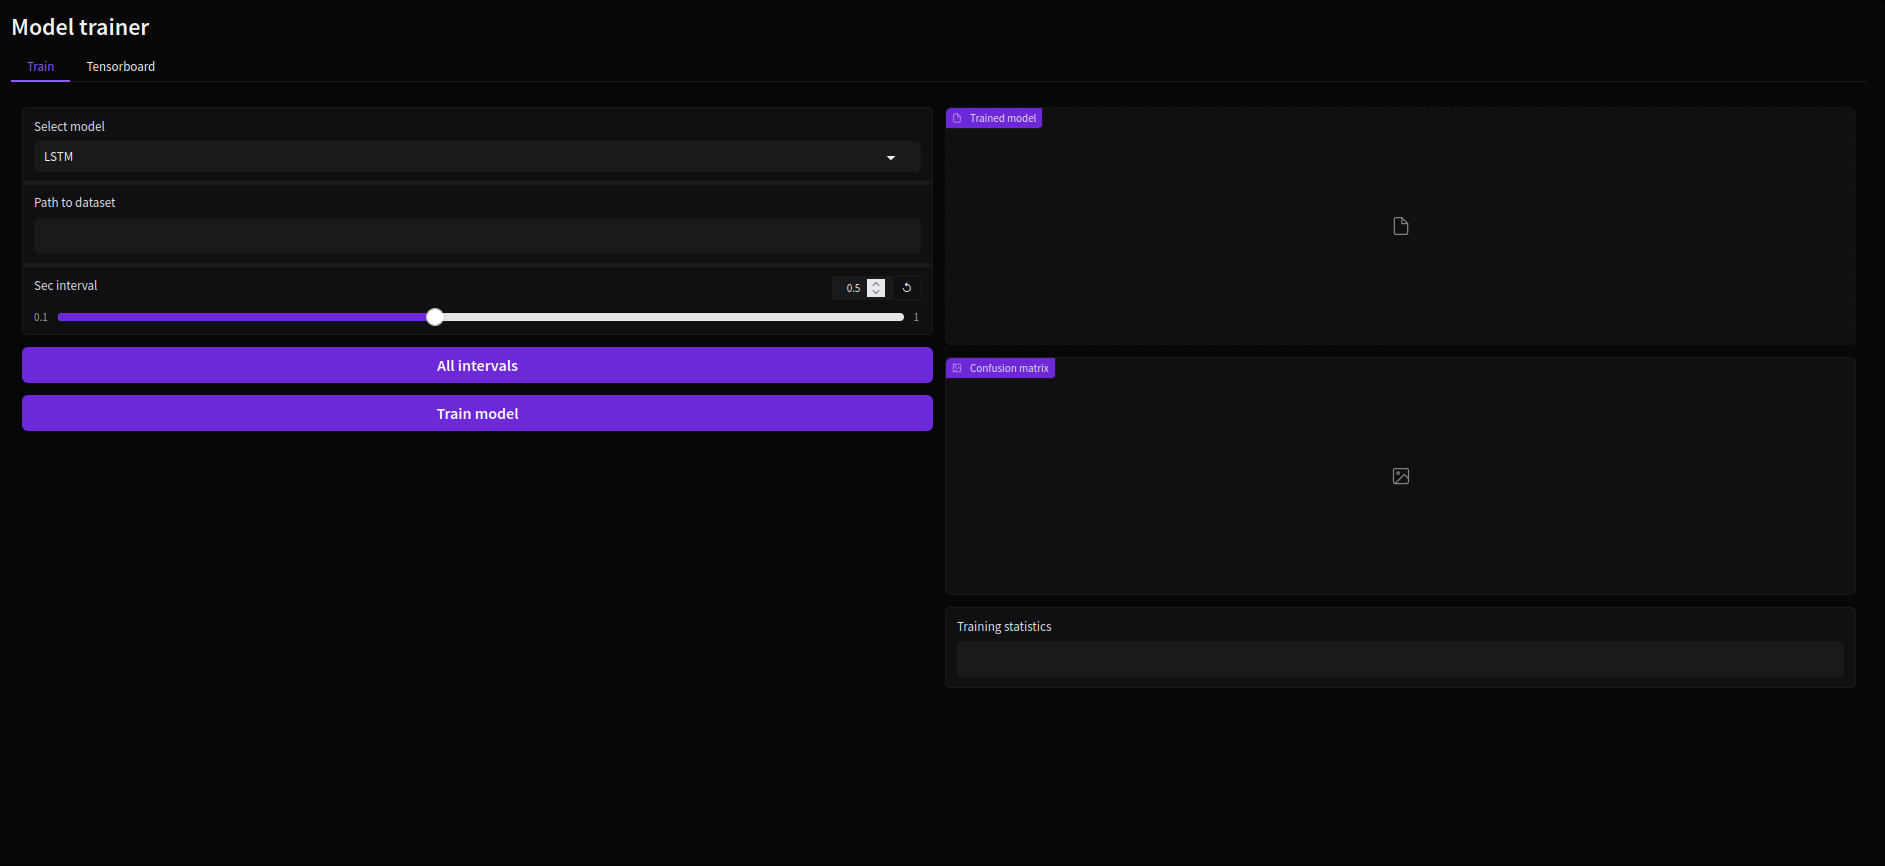
\includegraphics[width=0.9\textwidth]{Imagenes/Bitmap/interfaz-train.png}
    \caption{Interfaz de entrenamiento}
    \label{fig:interfaz-train}
\end{figure}


La función de entrenamiento que se ejecuta al pulsar el botón ``Train model'' hace lo siguiente:
\begin{enumerate}
    \item Se crea un entrenador del modelo seleccionado
    \item Se crea un objeto \textit{DataLoader} que se encargará de cargar los datos con el intervalo de tiempo de separación seleccionado.
    \item Se separan los datos cargados en 60\% para entrenamiento, 20\% para validación y 20\% para test.
    \item Se pasan las categorías con \textit{LabelEncoder} para que el modelo pueda entenderlas.
    \item Se entrena el modelo con los datos de entrenamiento y validación.
    \item Se guarda el modelo.
    \item Se comprueba cual es el mejor modelo entrenado entre todos los intervalos de tiempo seleccionados.
    \item Se muestra la matriz de confusión en la interfaz, el archivo del modelo y sus estadisticas.
\end{enumerate}

En la parte superior izquierda se puede ver dos secciones: ``Train'' y ``TensorBoard''. La sección ``Train'' es la explicada anteriormente, la sección ``TensorBoard'' es una sección que permite ver el progreso del entrenamiento en tiempo real. No solo eso, sino que también nos permite ver el rendimiento de modelos ya entrenados y ver como los hiperparámetros han afectado a su tasa de acierto. TensorBoard permite añadir funciones al código de entrenamiento para modificar el comportamiento del método de entrenamiento y dejar constancia de las distintas partes del mismo. Esta interfaz se puede ver en la figura \ref{fig:interfaz-tensorboard}.

\begin{figure}[h!]
    \centering
    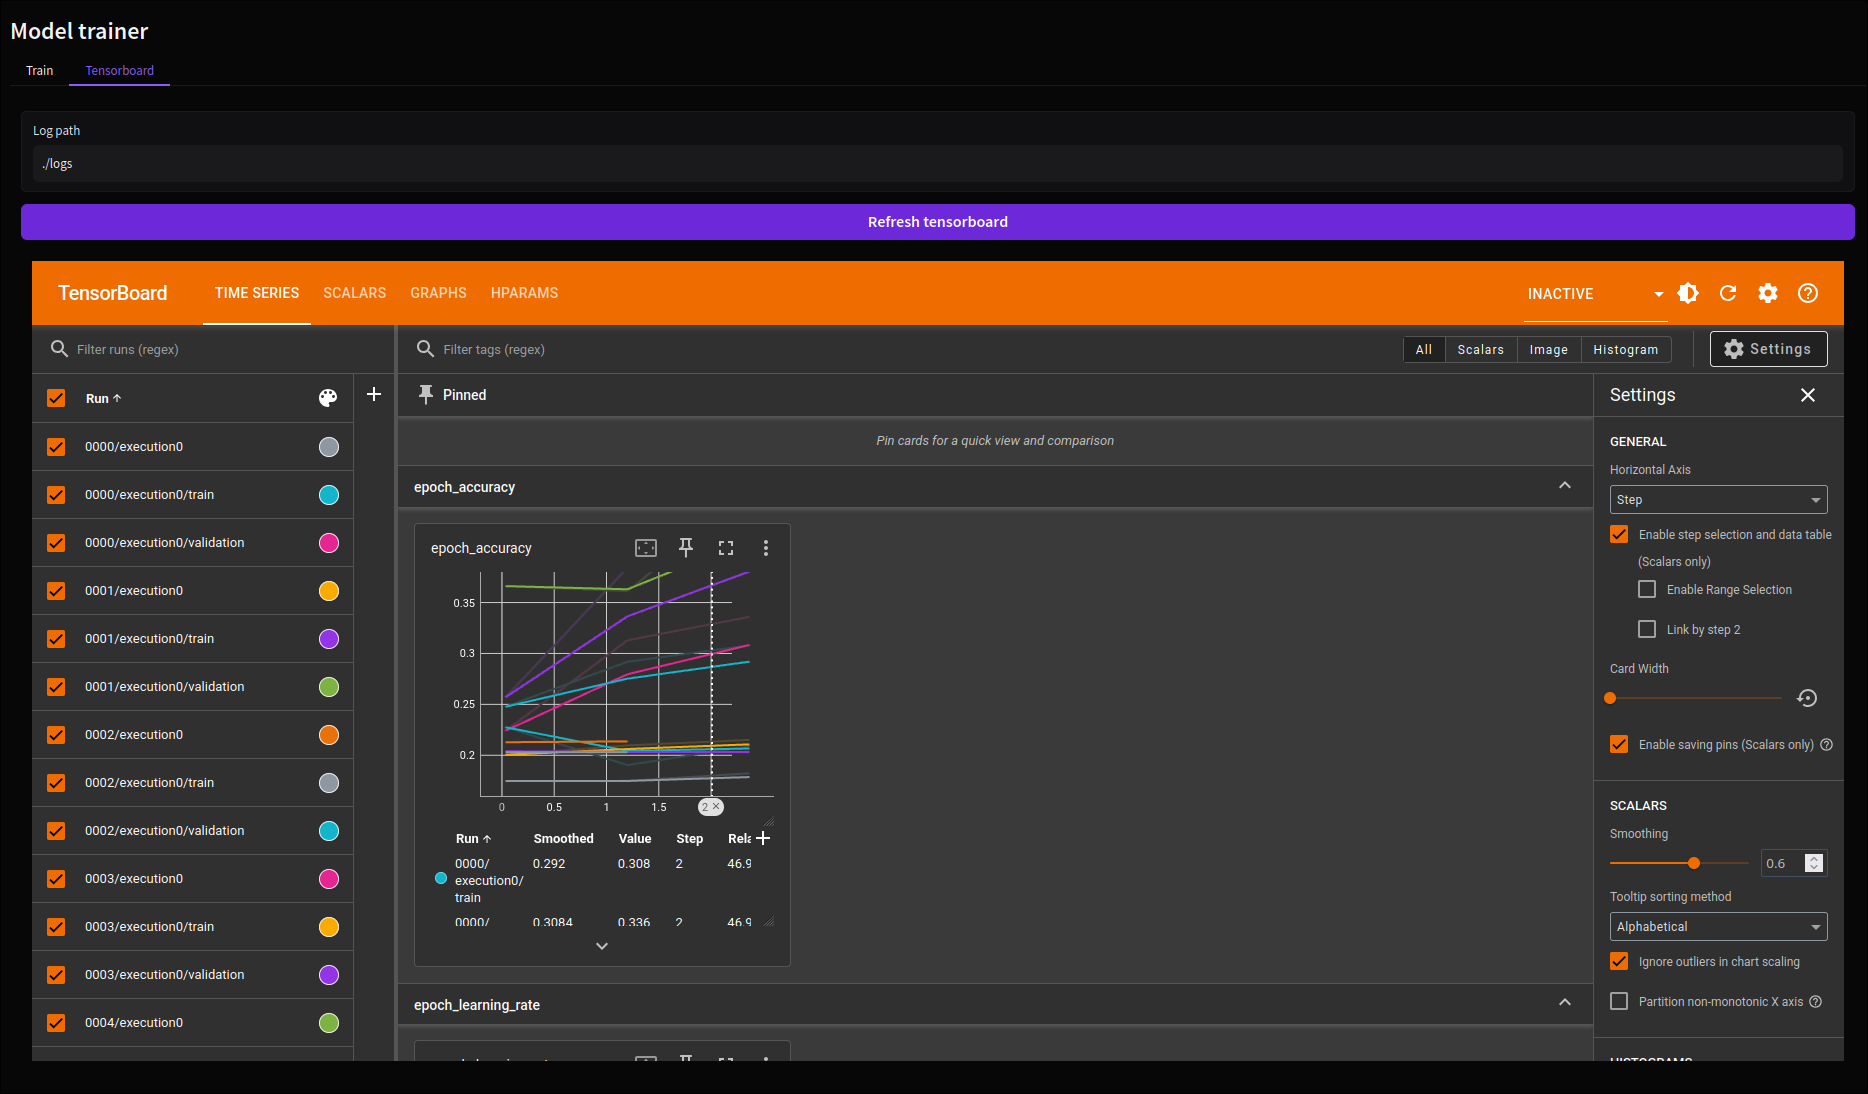
\includegraphics[width=0.9\textwidth]{Imagenes/Bitmap/interfaz-tensorboard.png}
    \caption{Interfaz de TensorBoard}
    \label{fig:interfaz-tensorboard}
\end{figure}

Para todo lo descrito, el archivo ``Interface.py'' tiene la estructura presentada en la figura \ref{fig:interfaz-estructura}. Las funciones \_\_change\_interval y \_\_change\_interval\_all cambian los intervalos de tiempo usados dentro del entrenamiento, \_\_setup\_ui crea el \textit{layout} de la interfaz, \_\_refresh\_tensorboard cambia la ruta de los \textit{logs} de TensorBoard y recarga el \gls{iframe}. El método \_\_train ejecuta todo el proceso de entrenamiento previamente descrito.

\begin{figure}[h!]
    \centering
    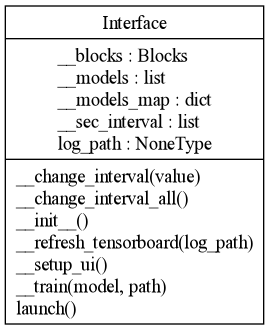
\includegraphics[width=0.3\textwidth]{Imagenes/Bitmap/classes_Interface.png}
    \caption{Estructura del archivo de la interfaz}
    \label{fig:interfaz-estructura}
\end{figure}

\subsection{Carga de datos}

La carga de datos se gestiona con la clase \textit{DataLoader}. Esta clase se mencionó en el apartado del dataset artificial ya que es la misma que se encarga de estandarizar los datos. Cuando se llama a la función de inicio de la clase se le pasa un intervalo de tiempo, este intervalo marca la distancia entre frames que se va a cargar. Si le indicamos una distancia de 0.8, cargará el frame 0 y el 72. Esto nos permite entrenar distintos modelos con distintas ventanas de envío de datos para comprobar si hay alguna diferencia en el rendimiento.

Estos datos una vez cargados se envían como una lista de tuplas <tipo\_animacion, lista\_de\_frames>. Tras esto, el objeto que reciba estos datos ya puede transformarlos como sea necesario y separarlos en entrenamiento, test y validación.

\subsection{Modelos usados}

A la hora de escoger modelos para la comparativa, se tuvo en cuenta el estudio \cite{combining3dskeleton} como un referente. Se tuvo siempre en cuenta que se intentaba buscar un modelo con el cómputo más simple posible para que fuera lo más accesible para cualquier tipo de máquina. Valorando también las dificultades de tiempo que conlleva el entrenamiento de modelos al final se consideró probar tres redes neuronales usadas para series temporales y un modelo clásico de clasificación.

En un primer momento se pensó también en modelos como \gls{yolo}, pero al ser un modelo basado en imágenes y el estudio plantearse con un traje de captura de movimiento, se decidió que sería una carga muy grande para las aplicaciones que usaran el modelo resultante por tener que renderizar una segunda cámara constantemente para el usuario. Otros modelos como \gls{svm} o \gls{knn} fueron descartados por falta de tiempo de entrenamiento.
\subsubsection{\gls{lstm}}

Este primer modelo va a servir para ilustrar como funcionan el resto de modelos basados en redes neuronales en este estudio. La estructura de la clase \textit{LSTMTrainer} se puede ver en la figura \ref{fig:lstm-estructura}. La mayoría de los atributos privados de la clase son los hiperparámetros del modelo, los otros atributos se usan para guardar información o para guardar el mecanismo usado para buscar hiperparámetros óptimos.

La función train\_with\_hparams se encarga de generar modelos con distintos hiperparámetros y entrenarlos para buscar el mejor. Para que este mecanismo fuera lo más eficiente posible, se ha hecho uso de la biblioteca keras-tuner (\cite{omalley2019kerastuner}), un \textit{framework} de búsqueda de hiperparámetros con distintos algoritmos de búsqueda ya implementados. Tras leer el arctículo \cite{li2018hyperbandnovelbanditbasedapproach} se optó por usar el algoritmo Hyperband, dado que los inconvenientes que presenta no representan un problema comparado con las ventajas de velocidad y eficiencia que otorga.

Esta búsqueda de hiperparámetros se centra en los siguientes:
\begin{itemize}
    \item \textbf{activation}: Función de activación de la capa oculta.
    \item \textbf{dropout}: Porcentaje de \textit{dropout} de la capa oculta.
    \item \textbf{recurrent\_activation}: Función de activación de la capa recurrente.
    \item \textbf{recurrent\_dropout}: Porcentaje de \textit{dropout} de la capa recurrente.
    \item \textbf{unroll}: Si se usa el \textit{unroll} de la capa LSTM.
    \item \textbf{use\_bias}: Si se usa el \textit{bias} de la capa LSTM.
\end{itemize}

El entrenamiento crea un modelo con los hiperparámetros seleccionados dentro de un rango, se entrena durante unas épocas y se comprueban resultados. Se pasa a otro conjunto de hiperparámetros y así hasta completarlos todos. Tras esto, se aumenta el número de épocas y se siguen entrenando los anteriores modelos. Tras acabar de entrenar todos los modelos, se selecciona el que mejor precisión en validación tenga.

De este ``mejor modelo'' se crea una matriz de confusión, se guarda el modelo en formato keras y se envían las estadísticas a la interfaz de gradio. Todo este proceso queda registrado en TensorBoard gracias a la lilbrería \textit{HParams} (\cite{hparams}).

\begin{figure}[h!]
    \centering
    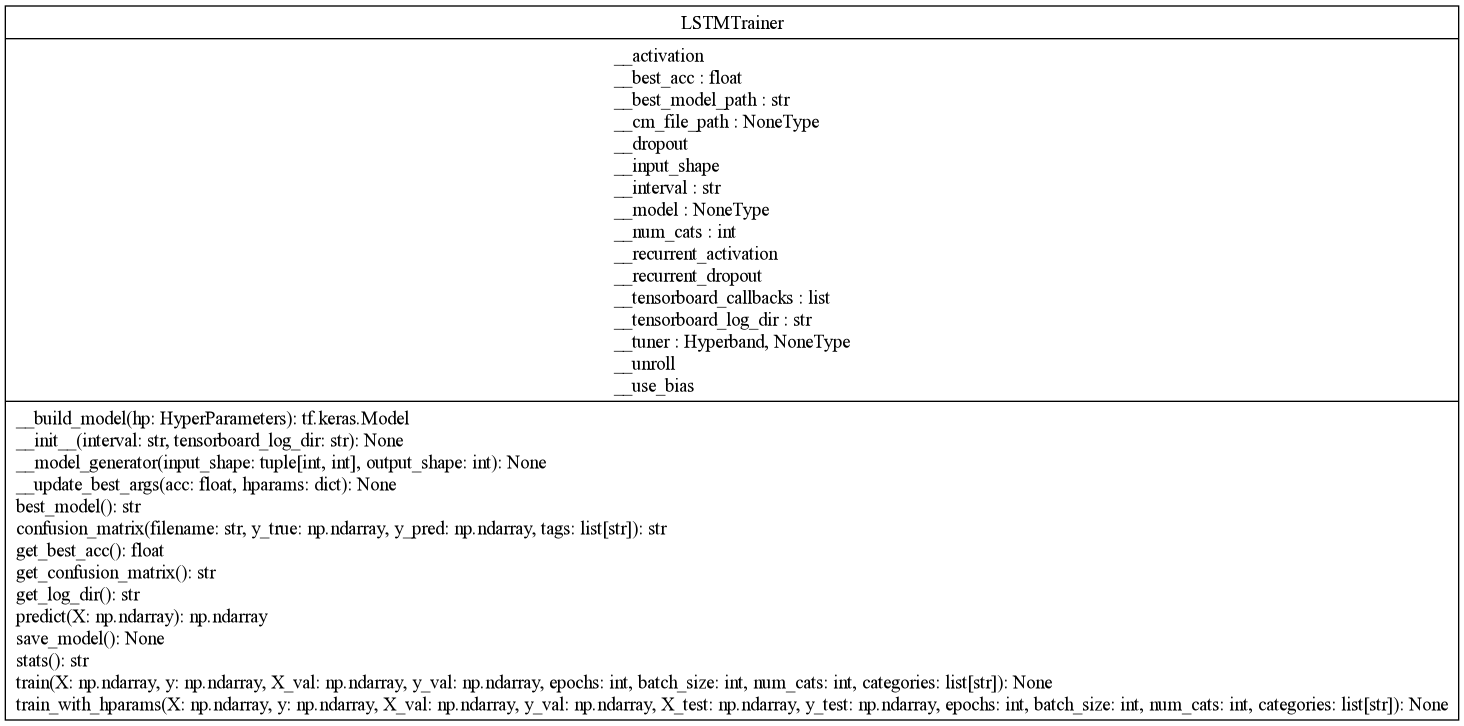
\includegraphics[width=0.8\textwidth]{Imagenes/Bitmap/classes_LSTMTrainer.png}
    \caption{Estructura de la clase LSTMTrainer}
    \label{fig:lstm-estructura}
\end{figure}

El modelo \gls{lstm} usado es un \textit{Sequential} de keras con una capa LSTM y una capa densa. La capa LSTM con los hiperparámetros antes descritos y la capa densa tiene tamaño el número de categorías de animaciones y una activación softmax. El modelo se compila utiliando el optimizador \textit{Adam}, la perdida se calcula con \textit{categorical\_crossentropy} y la métrica de evaluación es la \textit{accuracy}. Durante el proceso de entrenamiento se usan los \textit{callbacks} de \textit{EarlyStopping} para ahorrar recursos en entrenamientos que no parecen mejorar y los \textit{callbacks} de \textit{TensorBoard} para guardar los logs de entrenamiento y poder verlos en la interfaz de TensorBoard.

Entre los modelos de \gls{lstm} entrenados, el del intervalo de 0.8 fue el que mejor rendimiento tuvo, con una precisión de 0.5912 en validación. A continuación se puede ver el esquema del modelo en la figura \ref{fig:lstm-0.8-ejemplo}, la matriz de confusión en la figura \ref{fig:lstm-0.8-matriz-ejemplo} y el gráfico de entrenamiento en la figura \ref{fig:lstm-0.8-grafico-ejemplo}. Podemos ver en la matriz de confusión que los gestos menos reconocidos son baile y saludo. Los resultados del resto de intervalos se pueden ver en el apéndice \ref{appendix:resultadosLSTM}.

\begin{figure}[h!]
    \centering
    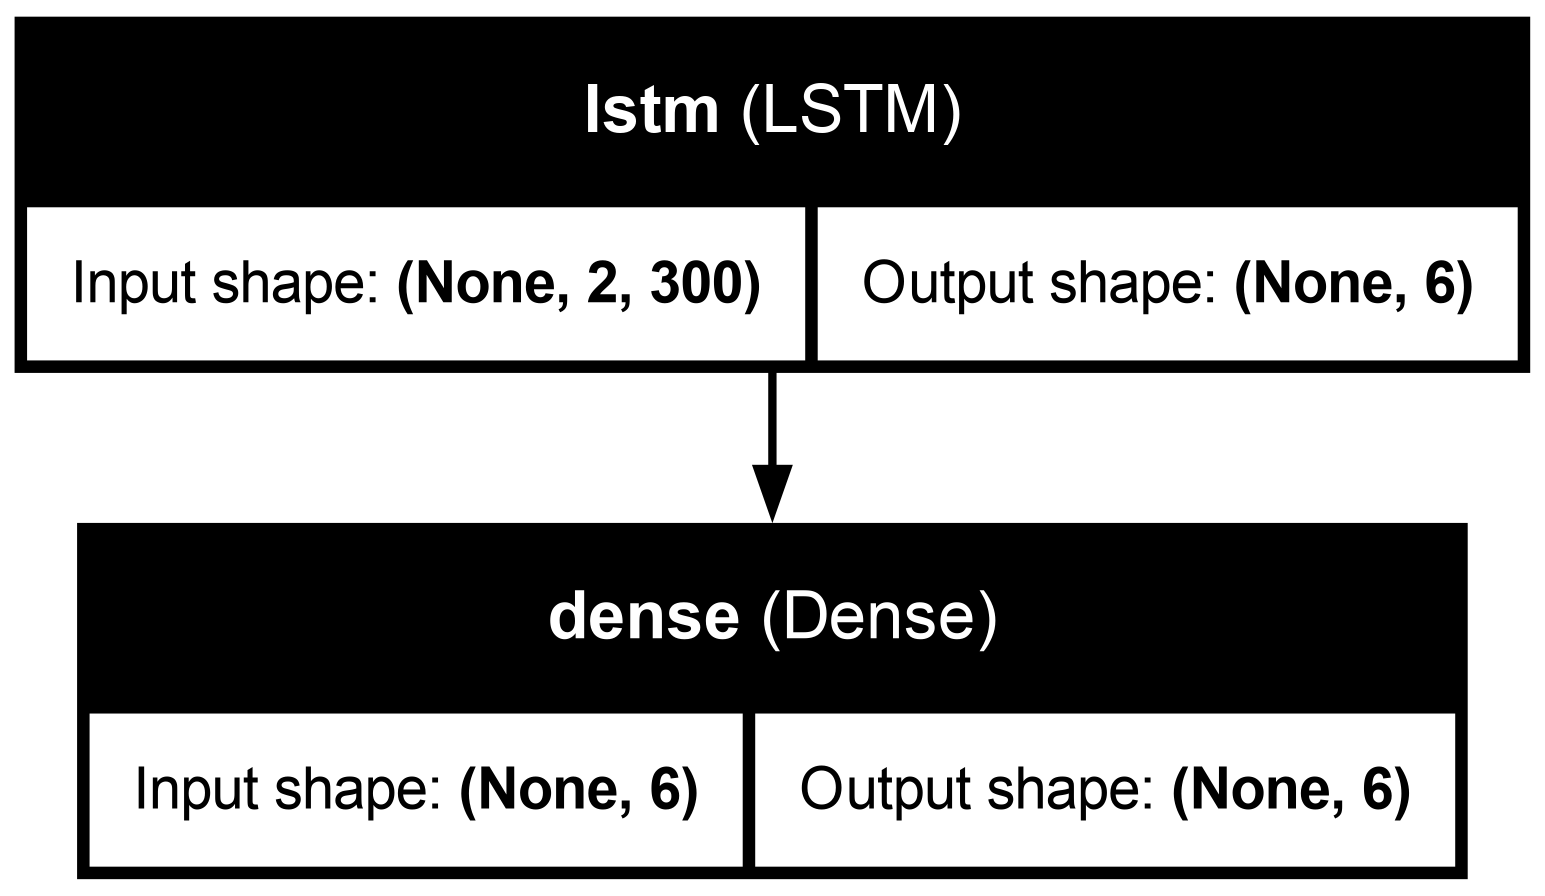
\includegraphics[width=0.8\textwidth]{Imagenes/Bitmap/best-lstm0.8.png}
    \caption{Esquema del modelo LSTM}
    \label{fig:lstm-0.8-ejemplo}
\end{figure}
\begin{figure}[h!]
    \centering
    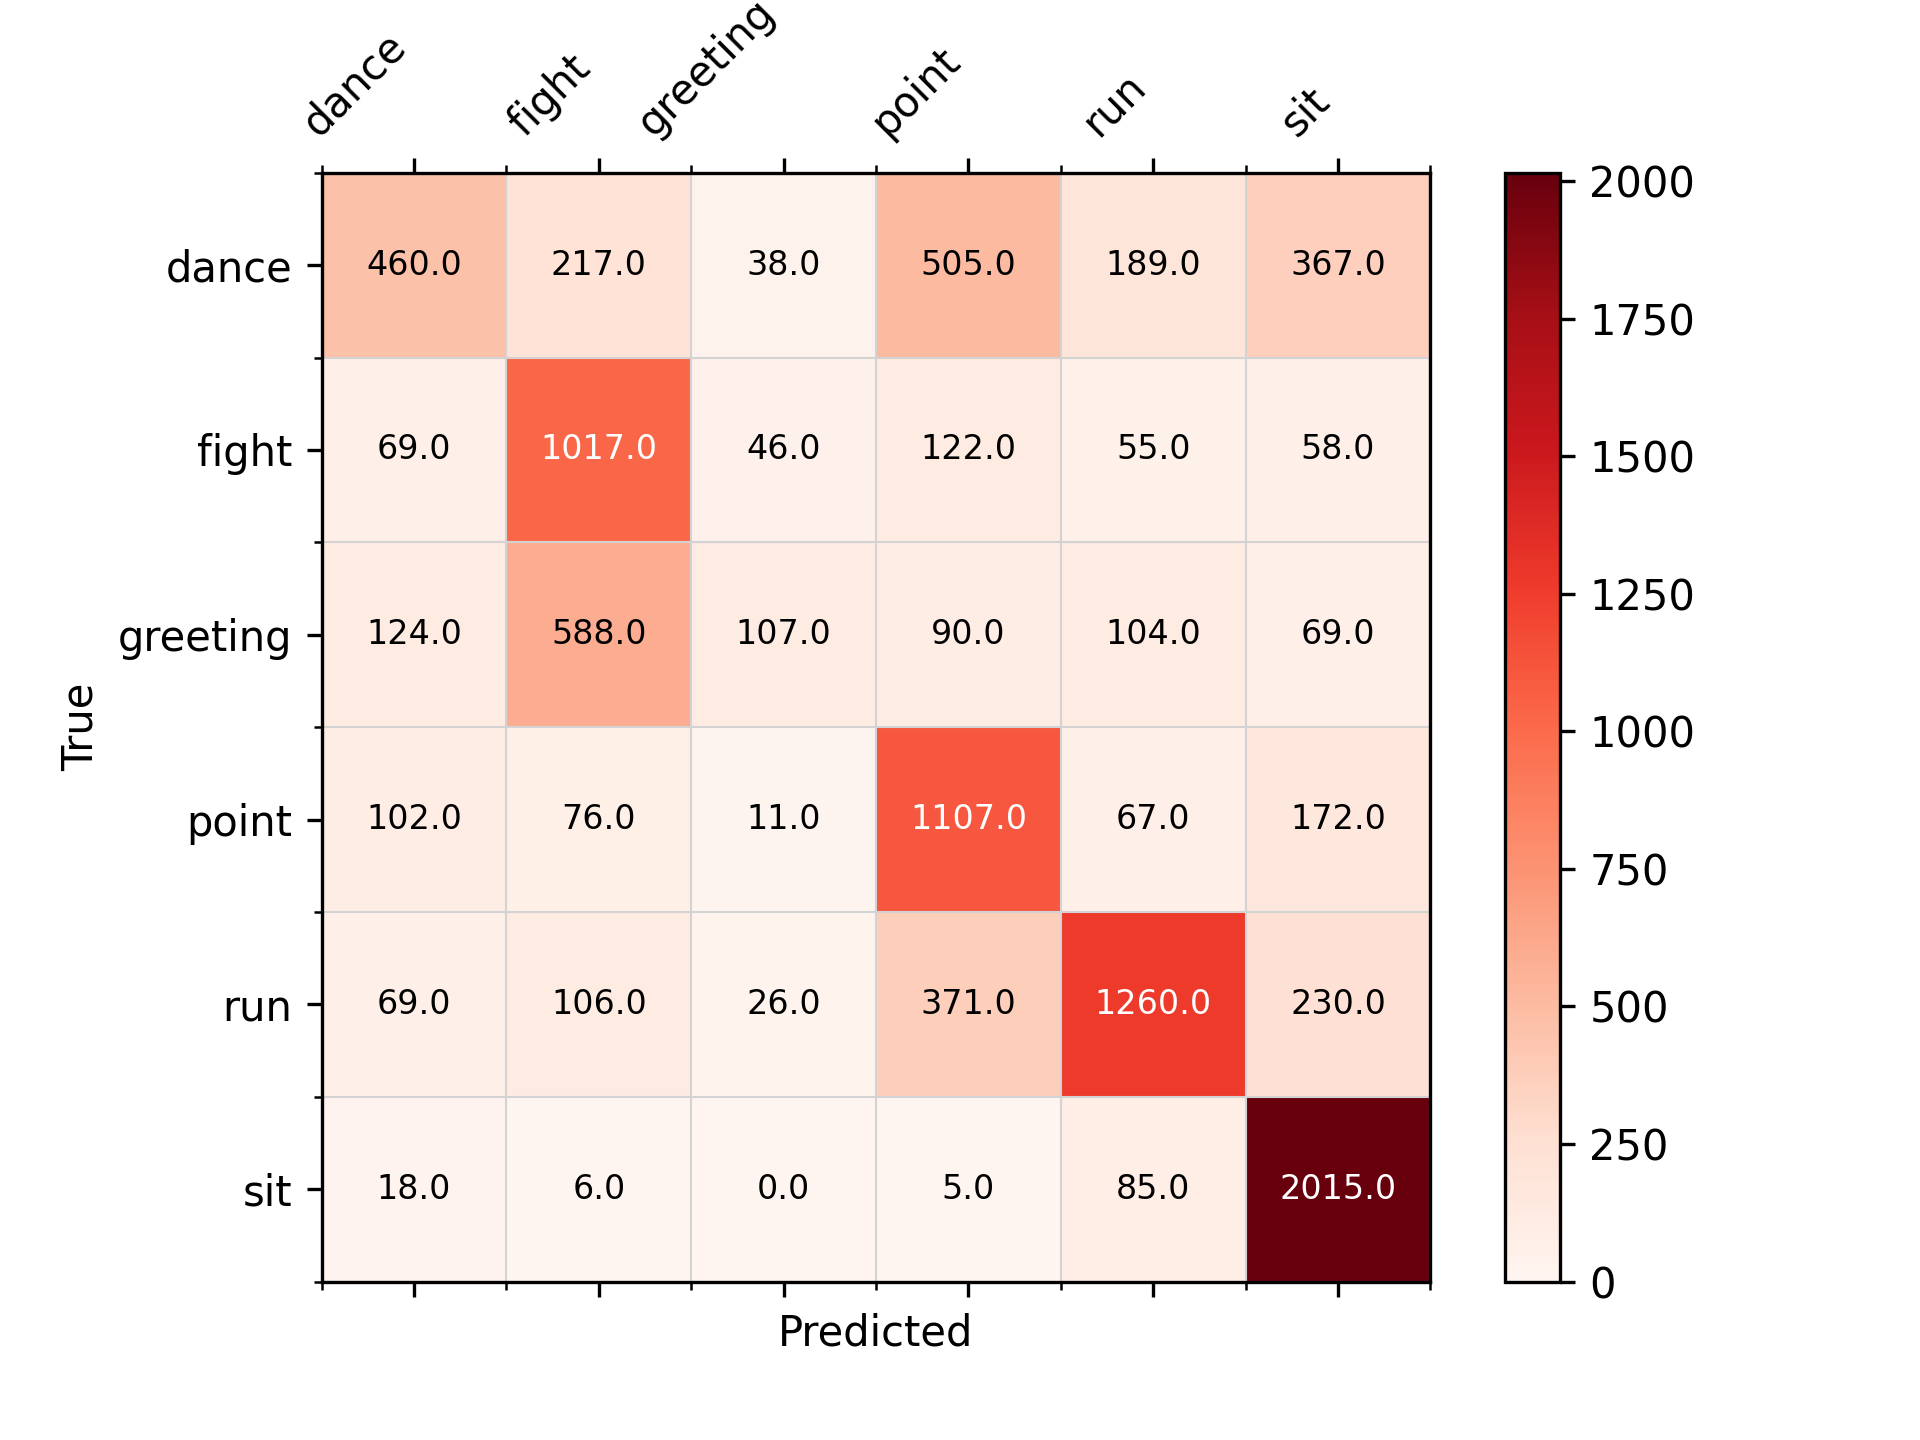
\includegraphics[width=0.8\textwidth]{Imagenes/Bitmap/CM_best-lstm0.8.png}
    \caption{Matriz de confusión del modelo LSTM}
    \label{fig:lstm-0.8-matriz-ejemplo}
\end{figure}
\begin{figure}[h!]
    \centering
    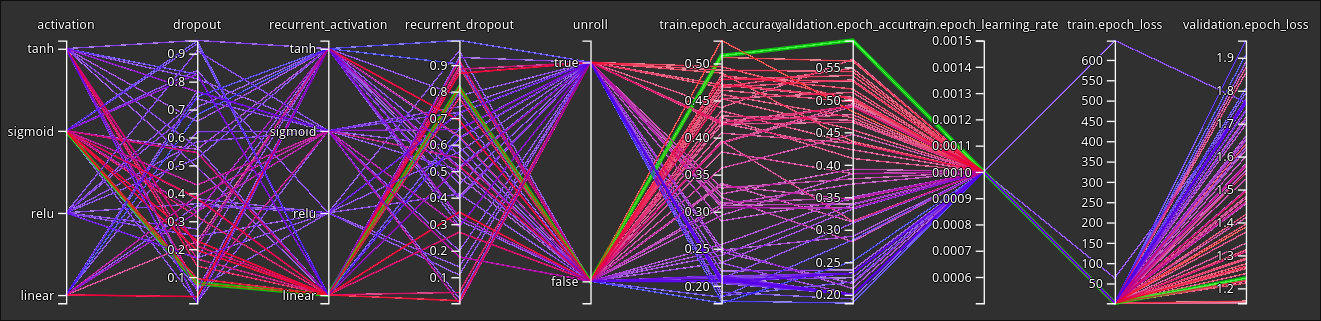
\includegraphics[width=0.8\textwidth]{Imagenes/Bitmap/tb-lstm-0.8.png}
    \caption{Gráfico de entrenamiento del modelo LSTM}
    \label{fig:lstm-0.8-grafico-ejemplo}
\end{figure}

\subsubsection{\gls{cnn}}


El modelo de \gls{cnn} se entrenó de una manera muy similar al de \gls{lstm}. En el uml de la figura \ref{fig:cnn-estructura} se puede ver la estructura de la clase \textit{CNNTrainer}, la cual es muy similar a la de \textit{LSTMTrainer}. La diferencia está en los hiperparámetros buscados. Estos son:
\begin{itemize}
    \item \textbf{activation}: Función de activación de la capa oculta.
    \item \textbf{conv\_filters}: Número de filtros de la capa convolucional.
    \item \textbf{dense\_units}: Número de neuronas de la capa densa.
    \item \textbf{dropout}: Porcentaje de \textit{dropout} de la capa oculta.
    \item \textbf{kernel\_size}: Tamaño del kernel de la capa convolucional.
    \item \textbf{pool\_size}: Tamaño del \textit{pooling} de la capa convolucional.
\end{itemize}

\begin{figure}[h!]
    \centering
    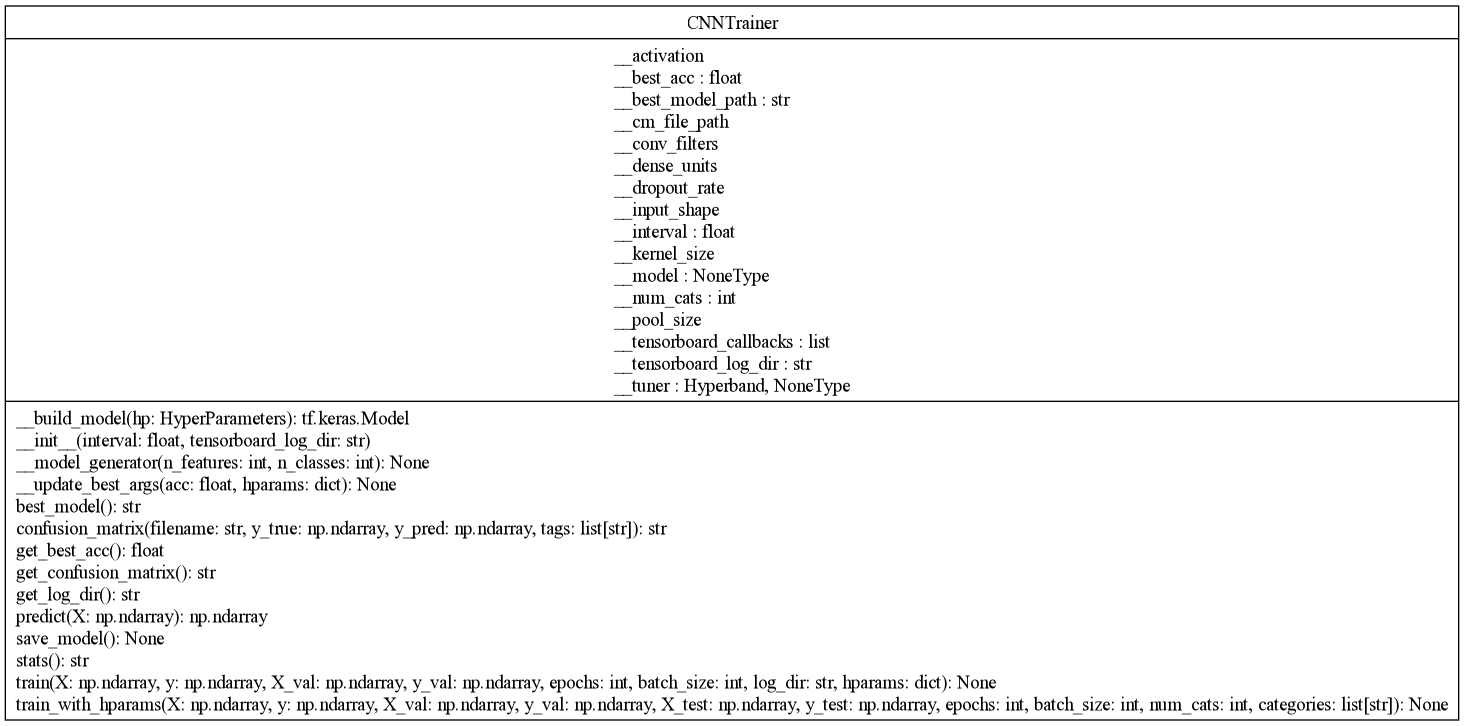
\includegraphics[width=0.8\textwidth]{Imagenes/Bitmap/classes_CNNTrainer.png}
    \caption{Estructura de la clase CNNTrainer}
    \label{fig:cnn-estructura}
\end{figure}

El método de entrenamiento es el mismo que el descrito en el apartado anterior, haciendo uso de keras-tuner para encontrar los mejores hiperparámetros. En el caso de este modelo, el mejor resultado se consigue con el intervalo de 1 segundo, haciendo este modelo más un reconocedor de poses que de gestos, con una precisión de 0.56002 en validación. La precisión en validación fue de 0.6342, lo que lo convierte en el mejor modelo entrenado. En la figura \ref{fig:cnn-1.0-ejemplo} se puede ver el esquema del modelo, en la figura \ref{fig:cnn-1.0-matriz-ejemplo} la matriz de confusión y en la figura \ref{fig:cnn-1.0-grafico-ejemplo} el gráfico de entrenamiento. En este caso podemos ver que los gestos que peor detecta son baile y saludo (siendo saludo muy confundido con pelea). Los resultados del resto de intervalos se pueden ver en el apéndice \ref{appendix:resultadosCNN}.
\begin{figure}[H]
    \centering
    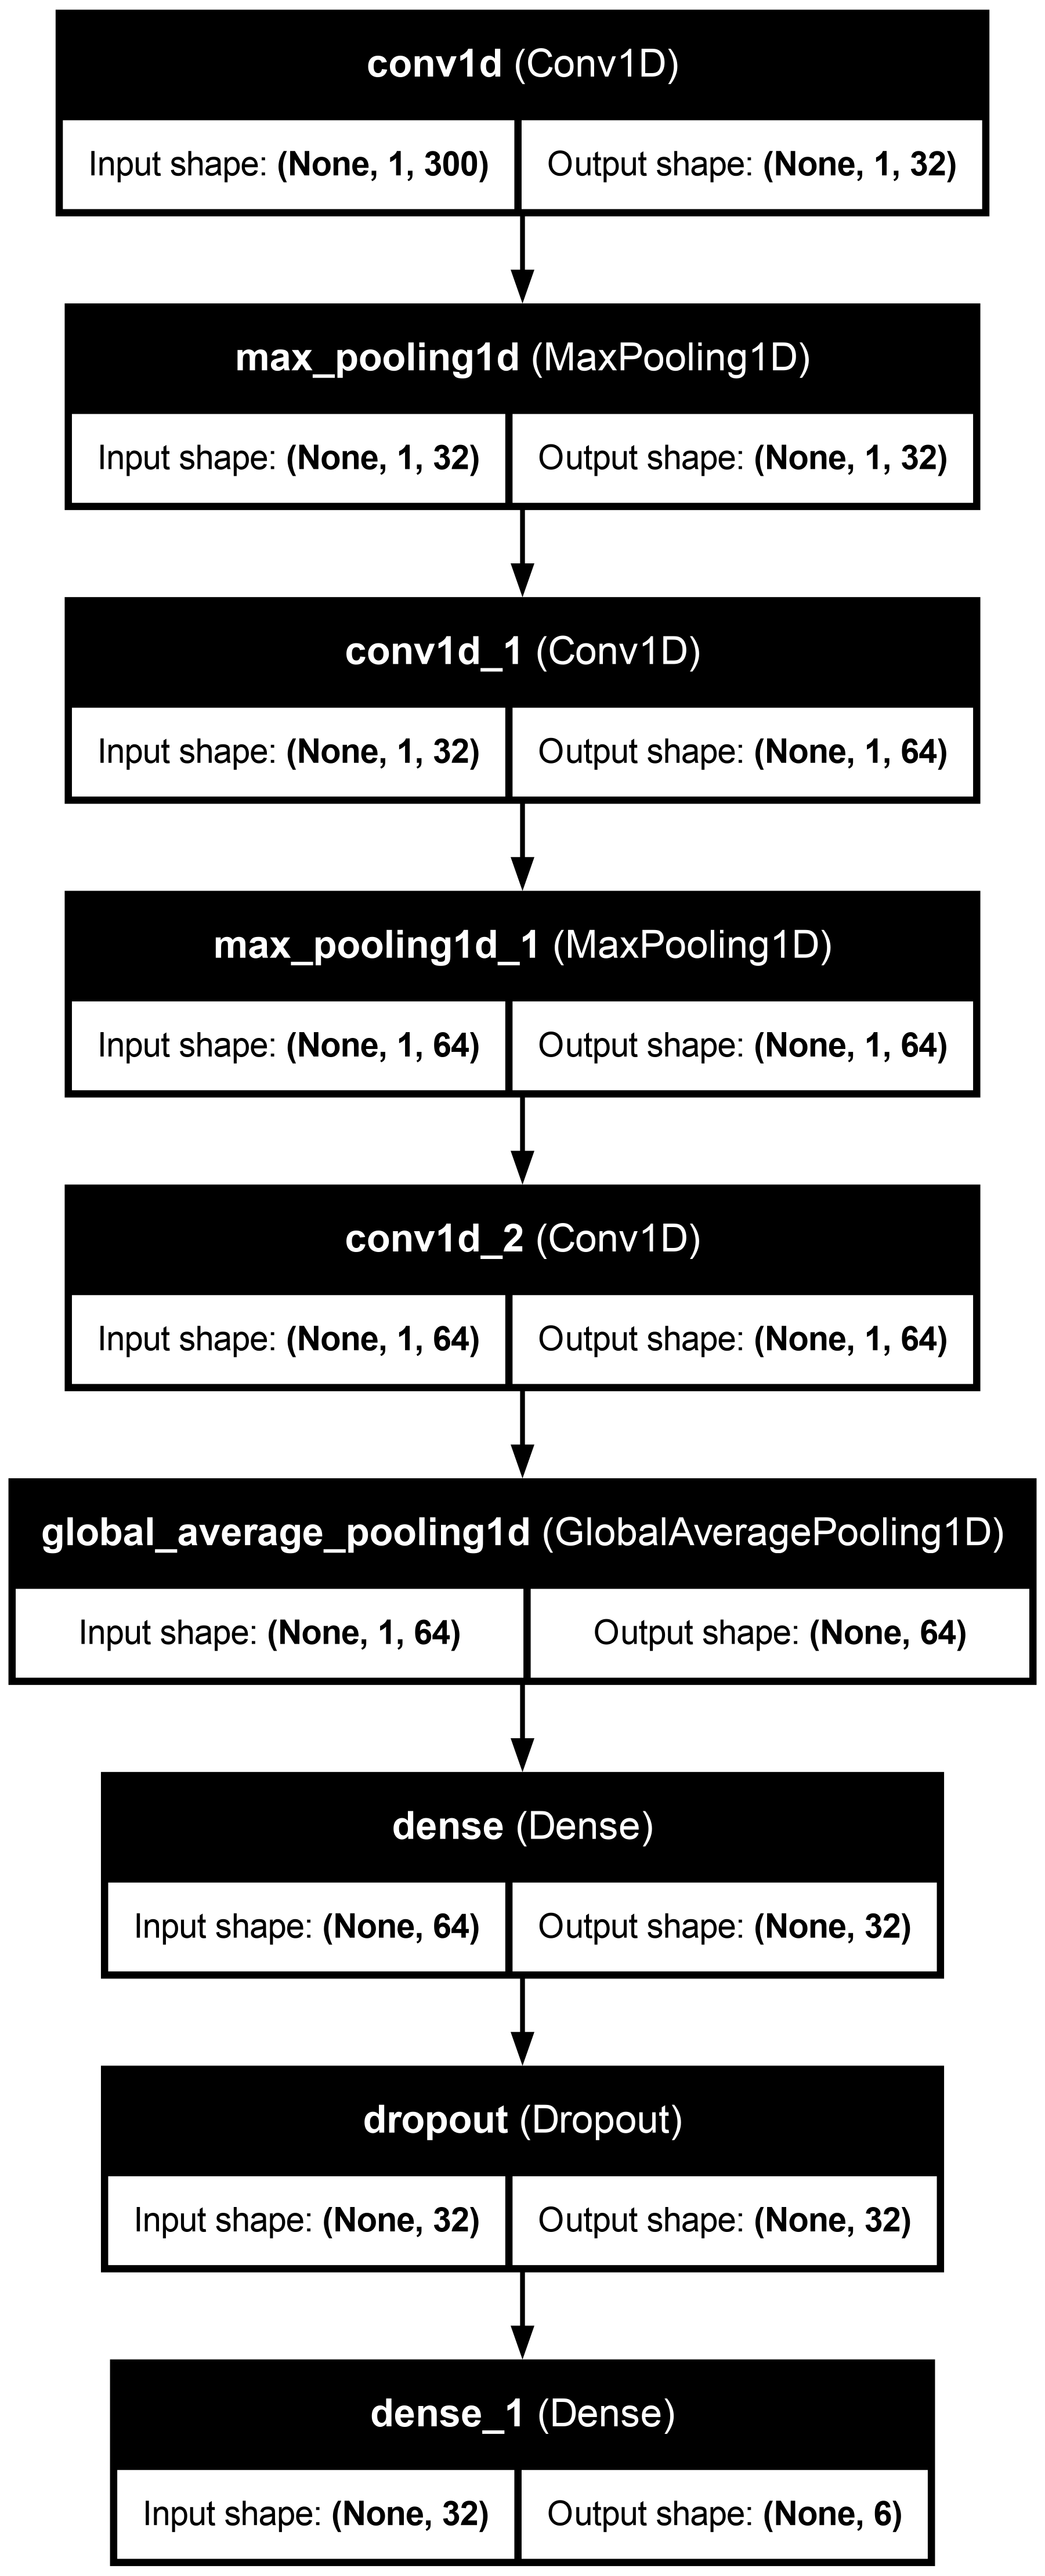
\includegraphics[width=0.3\textwidth]{Imagenes/Bitmap/best-cnn1.0.png}
    \caption{Esquema del modelo CNN}
    \label{fig:cnn-1.0-ejemplo}
\end{figure}

\begin{figure}[H]
    \centering
    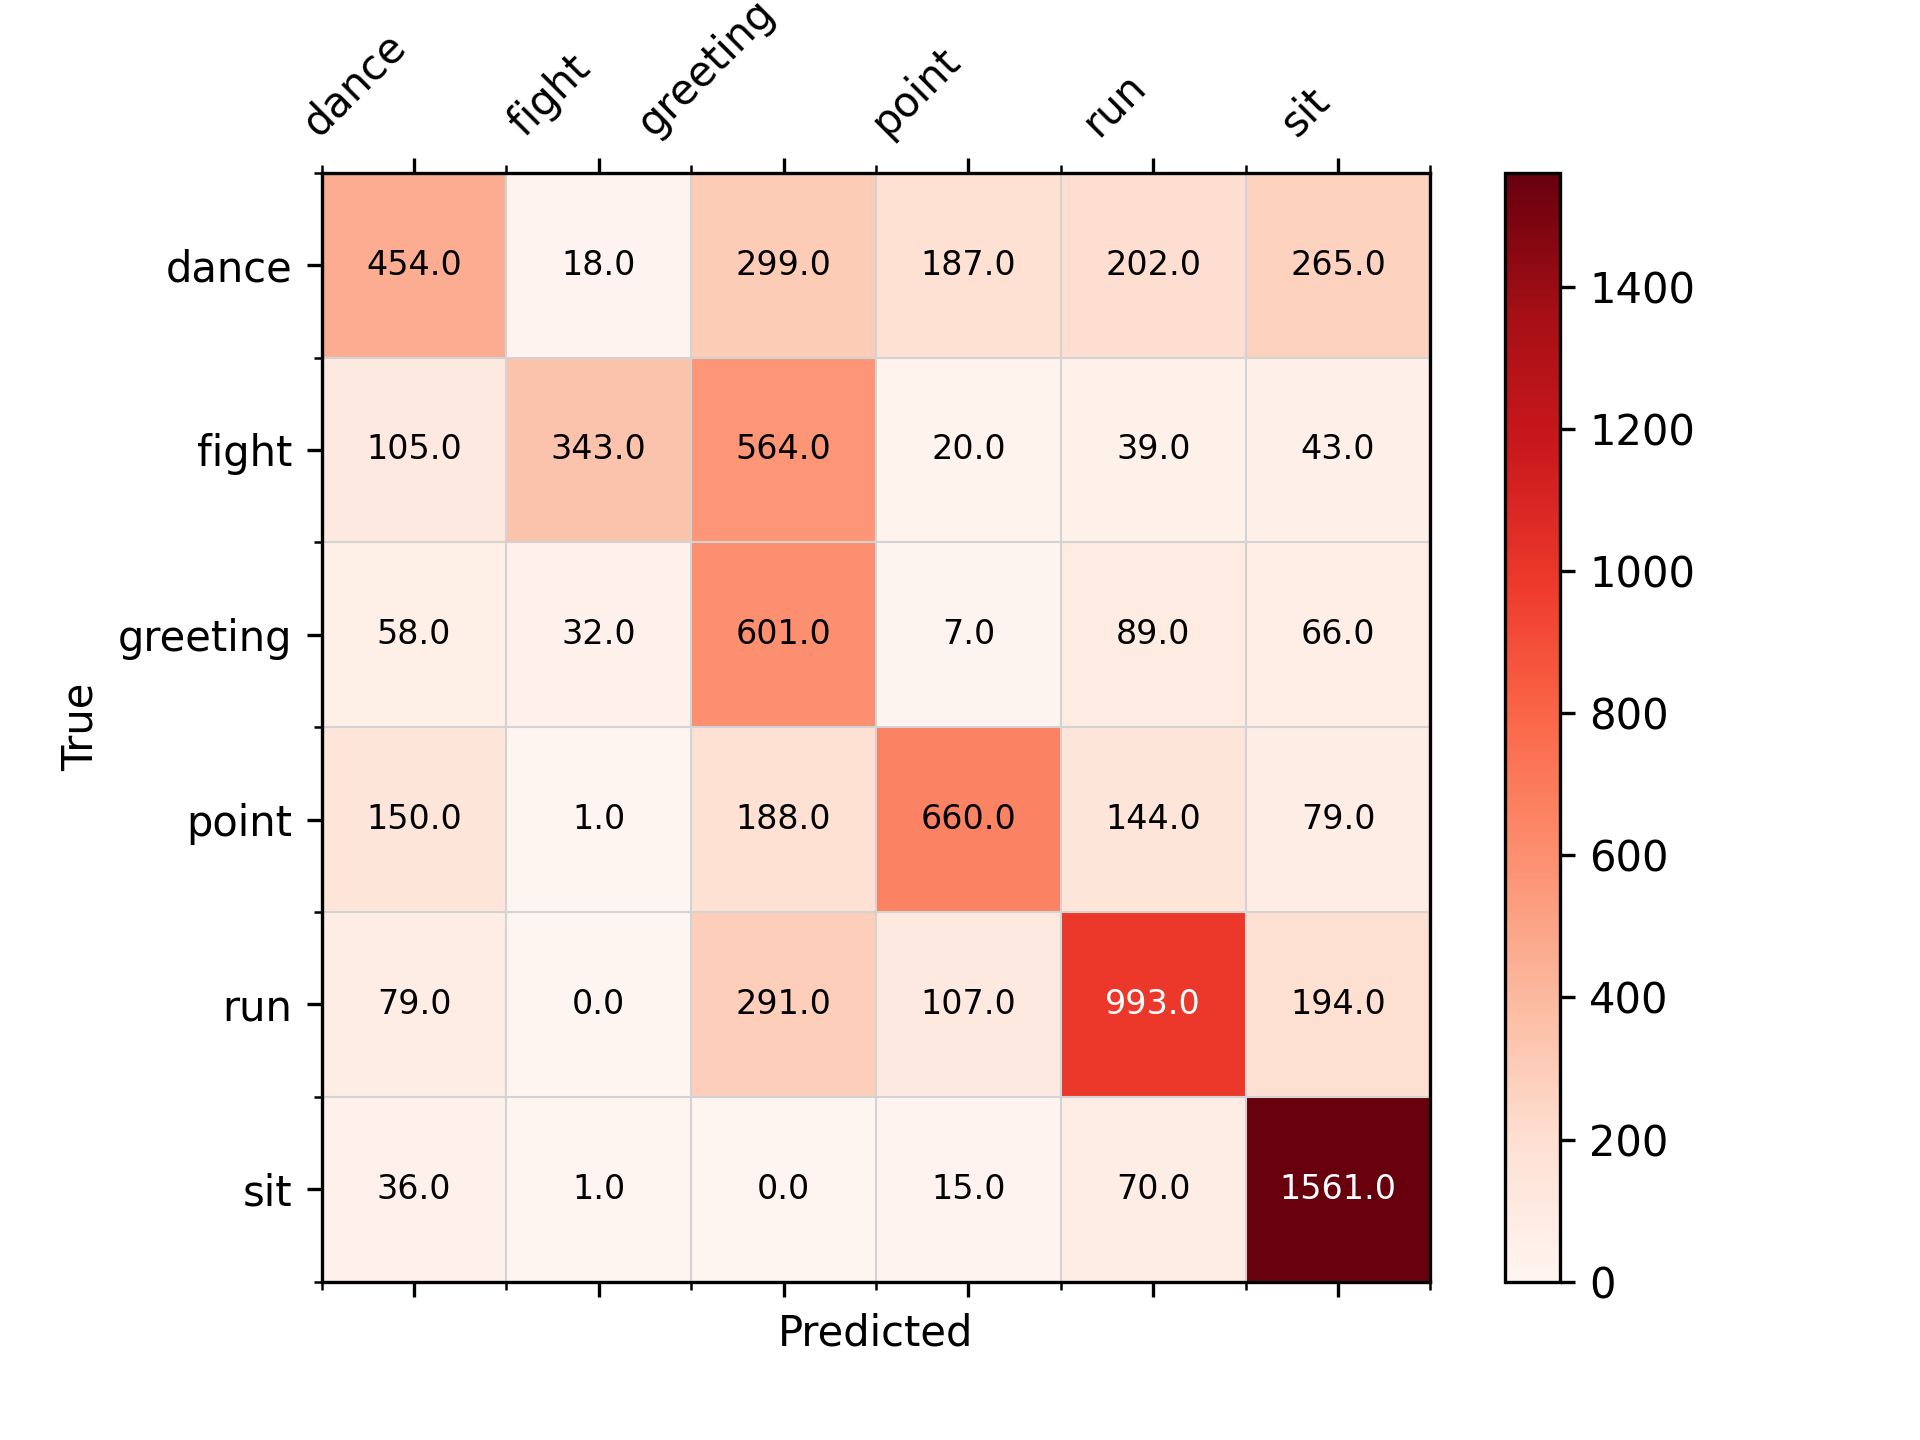
\includegraphics[width=0.6\textwidth]{Imagenes/Bitmap/CM_best-cnn1.0.png}
    \caption{Matriz de confusión del modelo CNN}
    \label{fig:cnn-1.0-matriz-ejemplo}
\end{figure}

\begin{figure}[H]
    \centering
    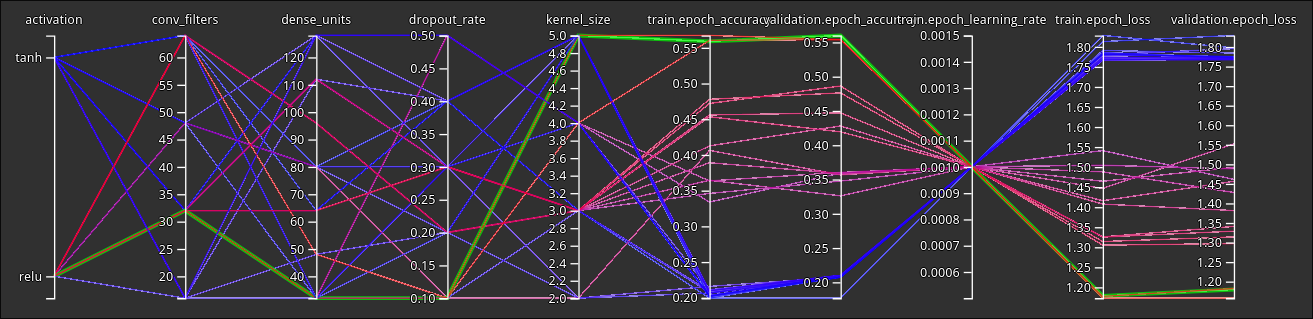
\includegraphics[width=0.8\textwidth]{Imagenes/Bitmap/tb-cnn-1.0.png}
    \caption{Gráfico de entrenamiento del modelo CNN}
    \label{fig:cnn-1.0-grafico-ejemplo}
\end{figure}

\subsubsection{\gls{rnn}}

Con el \gls{rnn} se sigue la misma base que para los dos modelos anteriores. La clase \textit{RNNTrainer} (estructura en la figura \ref{fig:rnn-estructura} )es muy similar a las anteriores, cambiando una vez más los hiperparámetros a buscar. En este caso son:

\begin{itemize}
    \item \textbf{activation}: Función de activación de la capa oculta.
    \item \textbf{activity regularizer}: Regularizador de la capa oculta.
    \item \textbf{bias constraint}: Restricción del \textit{bias} de la capa oculta.
    \item \textbf{bias initializer}: Inicializador del \textit{bias} de la capa oculta.
    \item \textbf{bias regularizer}: Regularizador del \textit{bias} de la capa oculta.
    \item \textbf{dropout}: Porcentaje de \textit{dropout} de la capa oculta.
    \item \textbf{kernel constraint}: Restricción del kernel de la capa oculta.
    \item \textbf{kernel initializer}: Inicializador del kernel de la capa oculta.
    \item \textbf{kernel regularizer}: Regularizador del kernel de la capa oculta.
    \item \textbf{recurrent constraint}: Restricción de la capa oculta.
    \item \textbf{recurrent dropout}: Porcentaje de \textit{dropout} de la capa oculta.
    \item \textbf{recurrent initializer}: Inicializador de la capa oculta.
    \item \textbf{recurrent regularizer}: Regularizador de la capa oculta.
    \item \textbf{unroll}: Si se usa el \textit{unroll} de la capa oculta.
    \item \textbf{use bias}: Si se usa el \textit{bias} de la capa oculta.
\end{itemize}

\begin{figure}[h!]
    \centering
    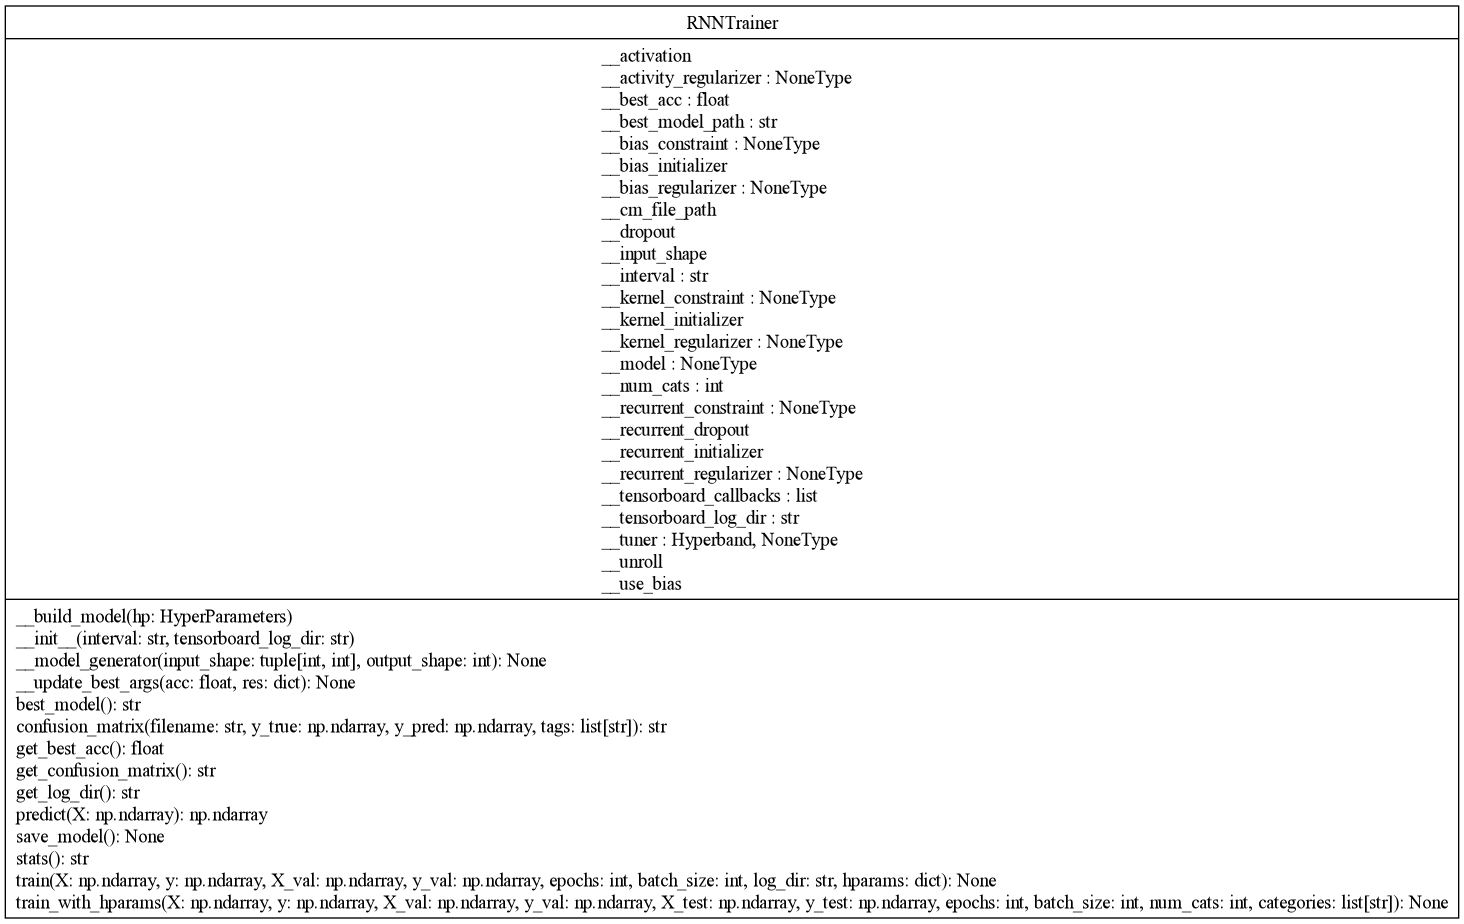
\includegraphics[width=0.8\textwidth]{Imagenes/Bitmap/classes_RNNTrainer.png}
    \caption{Estructura de la clase RNNTrainer}
    \label{fig:rnn-estructura}
\end{figure}

A pesar de ser el modelo con mayor busqueda de hiperparámetros, está en una reñida competición con el modelo \gls{cnn} para ver cual de los dos detecta peor los gestos. Su mejor intervalo ha sido el de 0.8 segundos con una precisión de 0.47865 en validación. En la figura \ref{fig:rnn-0.8-ejemplo} se puede ver el esquema del modelo, en la figura \ref{fig:rnn-0.8-matriz-ejemplo} la matriz de confusión y en la figura \ref{fig:rnn-0.8-grafico-ejemplo} el gráfico de entrenamiento. En este caso podemos ver que los gestos que peor detecta son baile y saludo (siendo pelea muy confundida con saludo). Los resultados del resto de intervalos se pueden ver en el apéndice \ref{appendix:resultadosRNN}.

\begin{figure}[H]
    \centering
    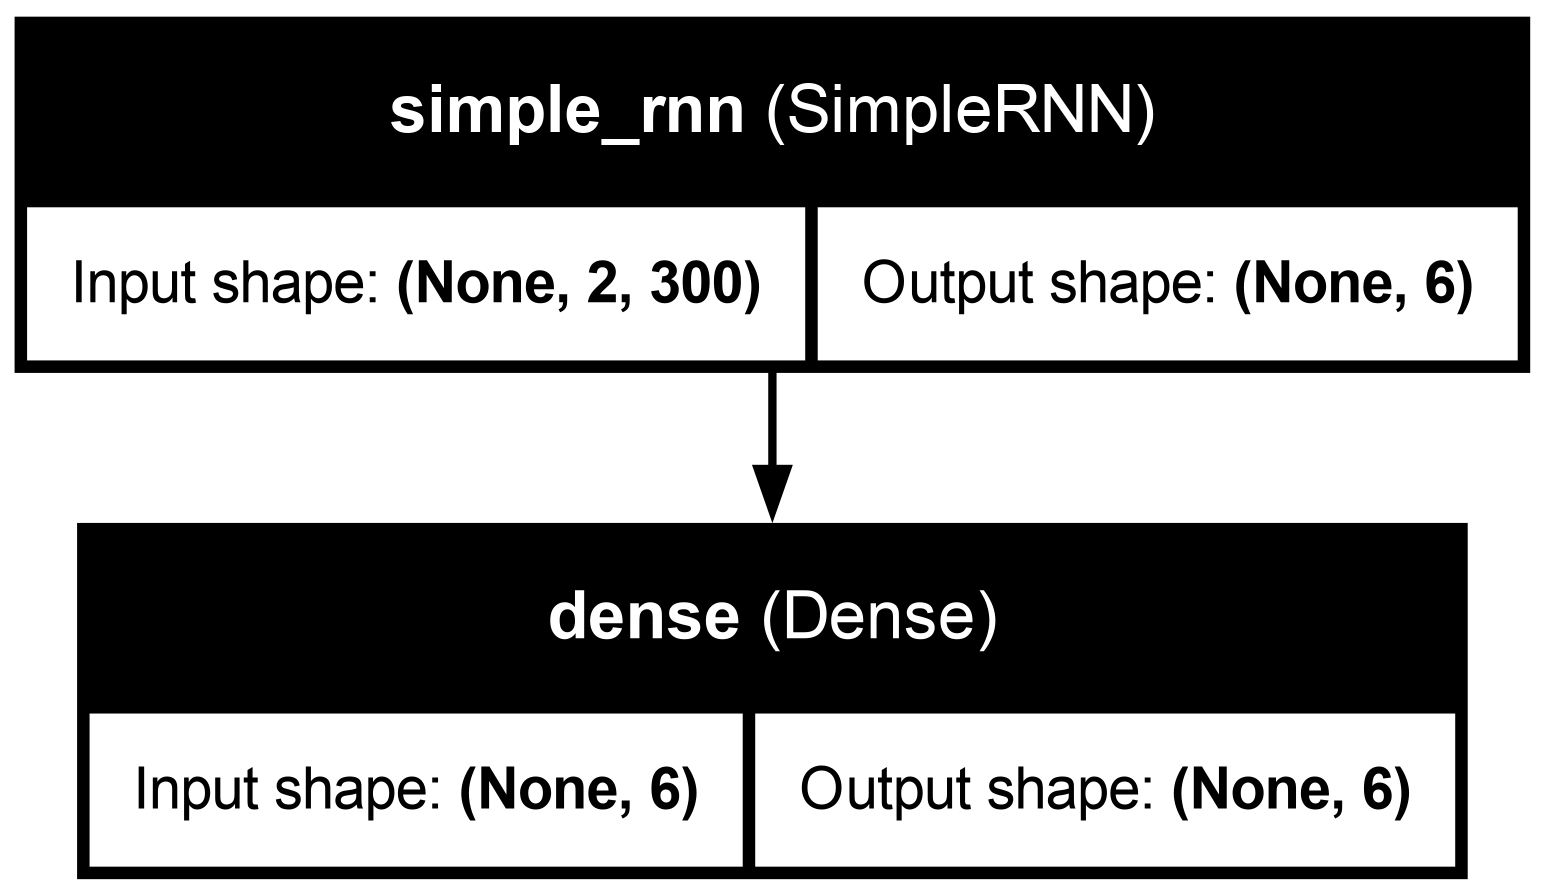
\includegraphics[width=0.3\textwidth]{Imagenes/Bitmap/best-rnn0.8.png}
    \caption{Esquema del modelo RNN}
    \label{fig:rnn-0.8-ejemplo}
\end{figure}

\begin{figure}[H]
    \centering
    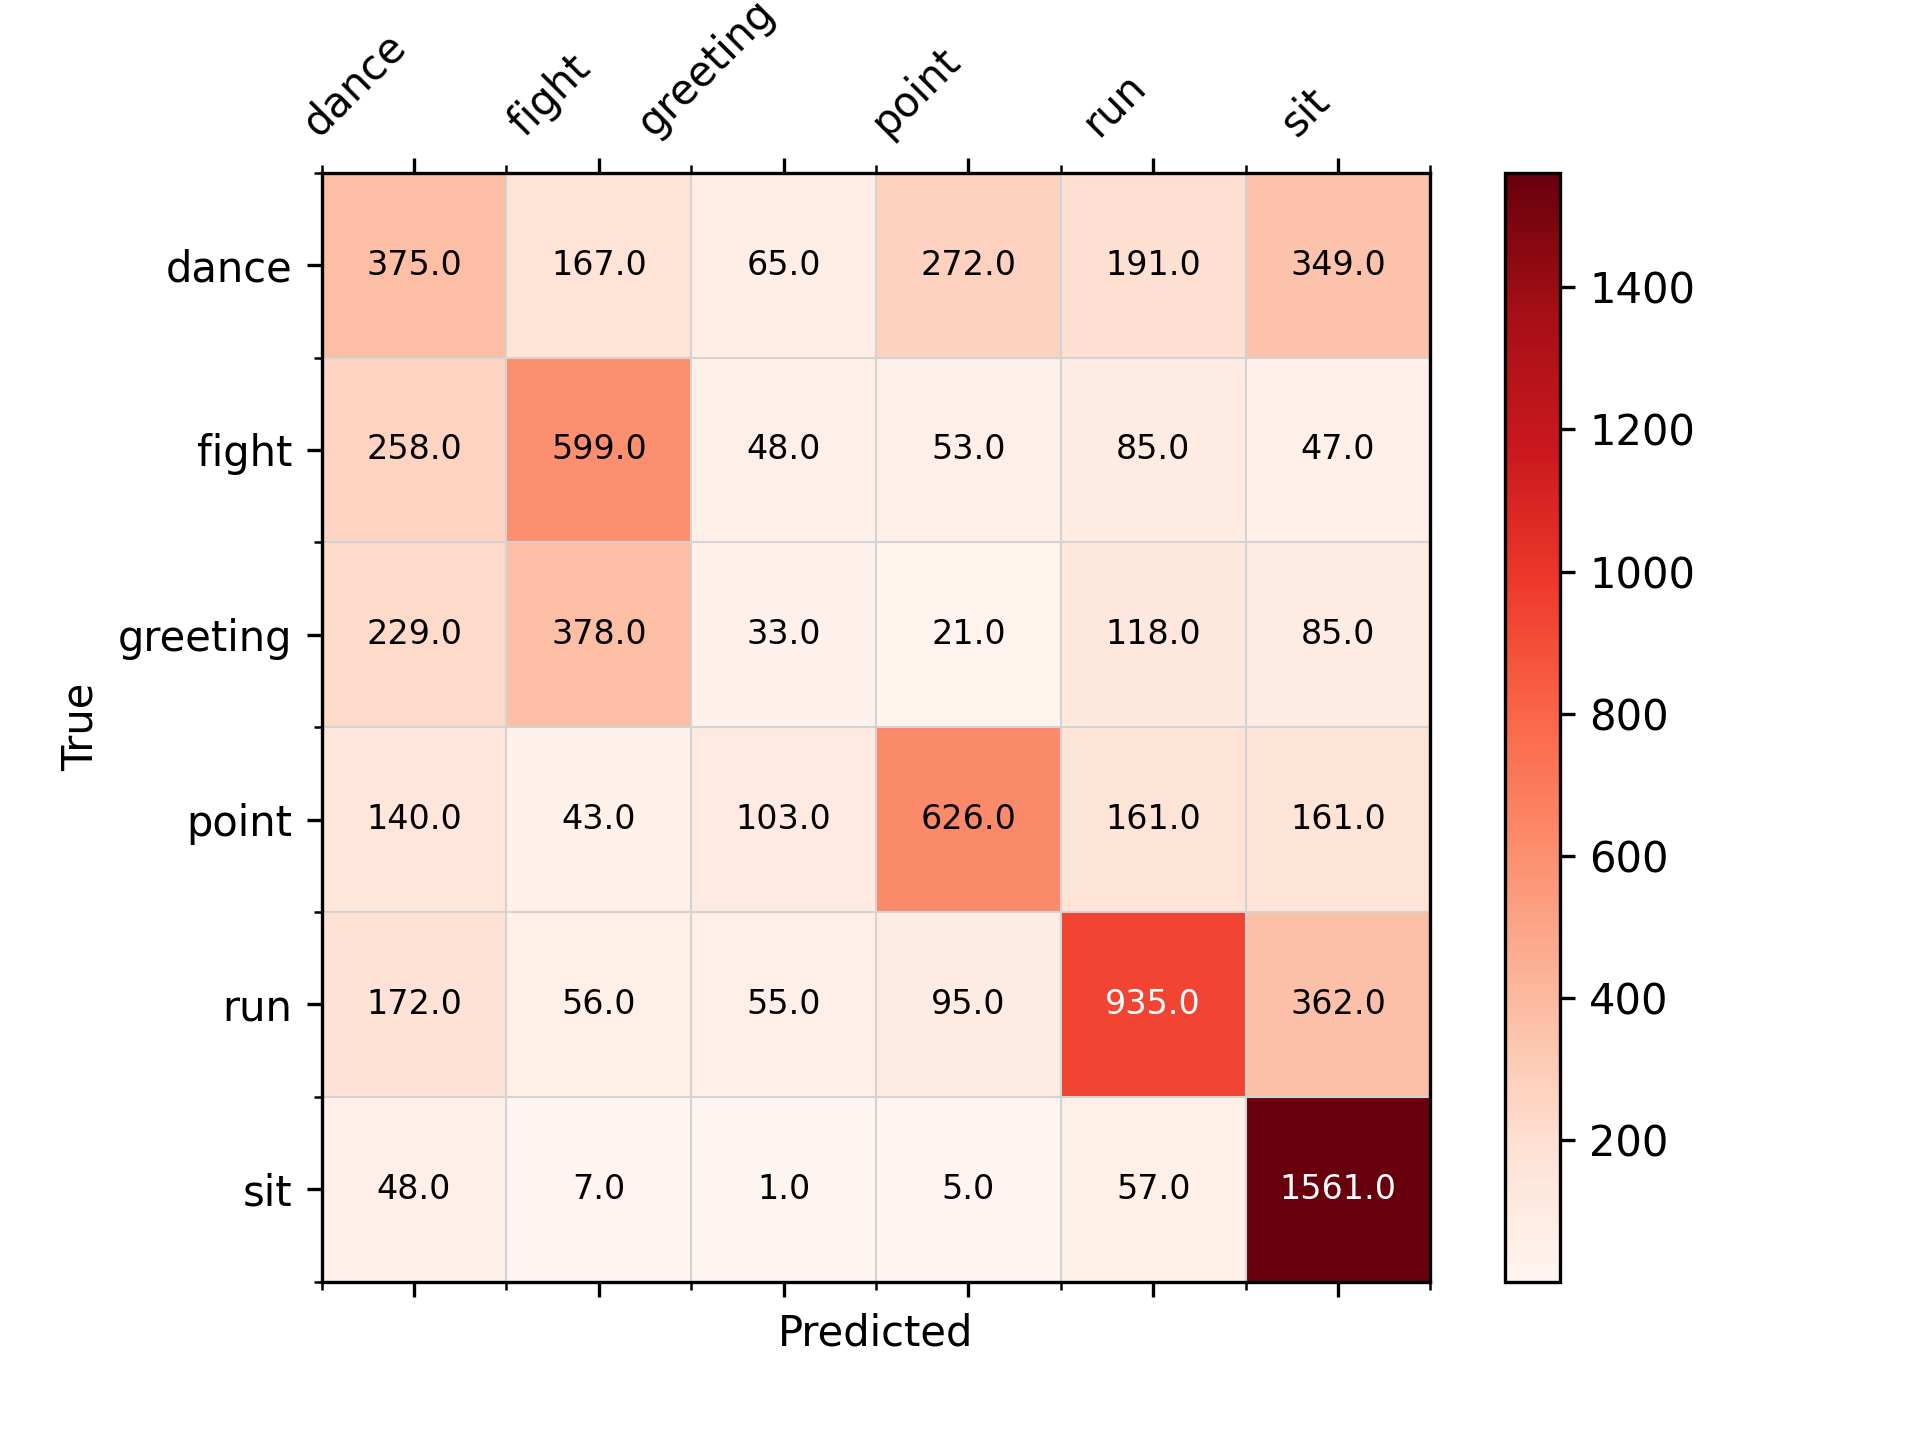
\includegraphics[width=0.6\textwidth]{Imagenes/Bitmap/CM_best-rnn0.8.png}
    \caption{Matriz de confusión del modelo RNN}
    \label{fig:rnn-0.8-matriz-ejemplo}
\end{figure}

\begin{figure}[H]
    \centering
    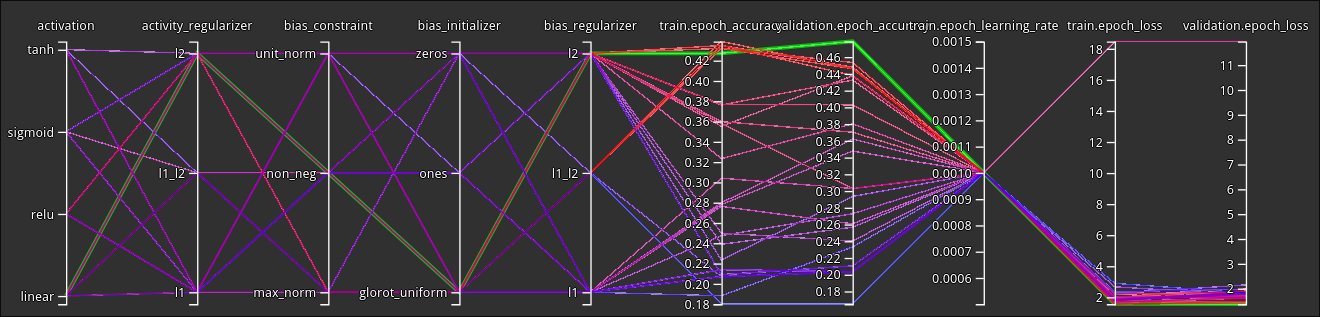
\includegraphics[width=0.8\textwidth]{Imagenes/Bitmap/tb-rnn-0.8.png}
    \caption{Gráfico de entrenamiento del modelo RNN}
    \label{fig:rnn-0.8-grafico-ejemplo}
\end{figure}

\subsubsection{\gls{randomforest}}

El entrenador del \gls{randomforest} es el más sencillo y el más distinto de todos. Este modelo no es una red neuronal, sino un modelo clásico de clasificación. La clase \textit{RandomForestTrainer} (estructura en la figura \ref{fig:rf-estructura}) sigue utilizando la función train\_with\_hparams como las anteriores aún no habiendo hparams como tal, haciendo esto se consigue mantener la igualdad de todas las clases de cara a la interfaz de gradio.

Este modelo no usa tensorflow como tal, dado que YDF es un desarrollo que deja atrás el uso de TensorFlow Decision Forest para implementar algoritmos más eficientes tanto en entrenamiento como en inferencia. A pesar de ser un desarrollo paralelo, el equipo de YDF decide hacer el modelo compatible con Tensorflow para poder integrarlo en un mayor ecosistema. Estos datos de mayor eficiencia se pueden comprobar en el estudio \cite{GBBSP23}.

A diferencia de los modelos anteriores, este modelo usa DataFrames de pandas para el entrenamiento y la predicción en vez de tensores. En este entrenamiento usamos \textit{RandomSearchTuner} para buscar la mejor combinación de número de árboles, profundidad máxima y mínimo de ejemplos.

\begin{figure}[h!]
    \centering
    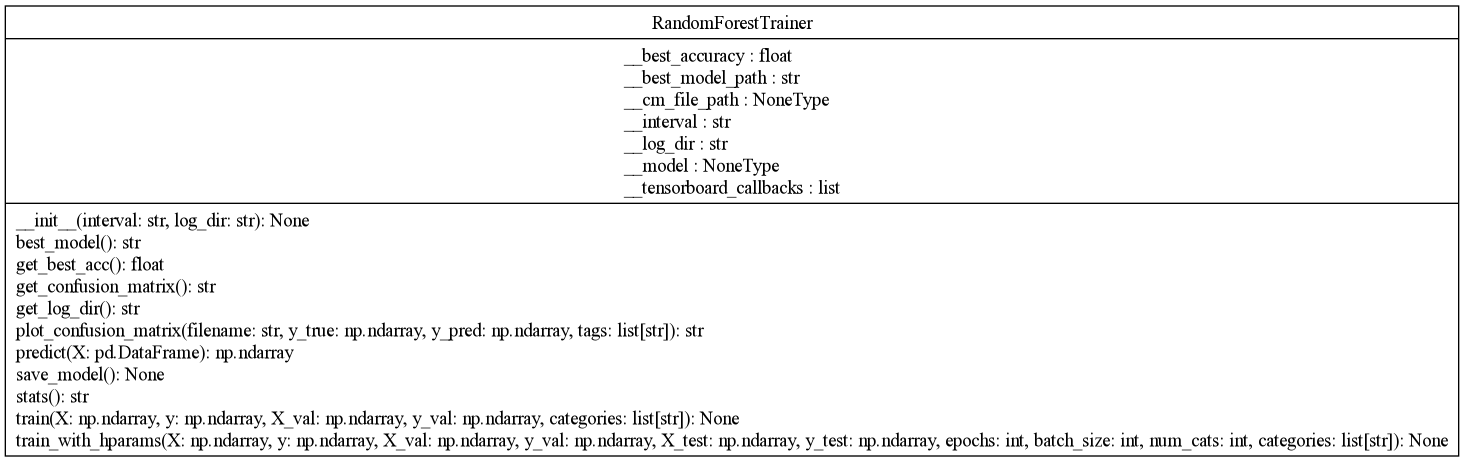
\includegraphics[width=0.8\textwidth]{Imagenes/Bitmap/classes_RandomForestTrainer.png}
    \caption{Estructura de la clase RFTrainer}
    \label{fig:rf-estructura}
\end{figure}

Por desgracia, este modelo no deja una constancia tan rigurosa como los anteriores dado que no usa TensorBoard ni tiene un equivalente. A pesar de esto, este es el modelo con mayor rendimiento de lejos. Todos los intervalos tienen un rendimiento más o menos equivalente, ganando el de 0.8 segundos por muy poco.

En la figura \ref{fig:rf-0.8-matriz-ejemplo} se puede ver la matriz de confusión del modelo y en el apendice \ref{appendix:resultadosRF} se pueden ver los resultados de todos los intervalos. En este caso podemos ver que los gestos que peor detecta son pelea y saludo. La precisión en validación fue de 0.85936, lo que lo convierte en el mejor modelo entrenado.

\begin{figure}[H]
    \centering
    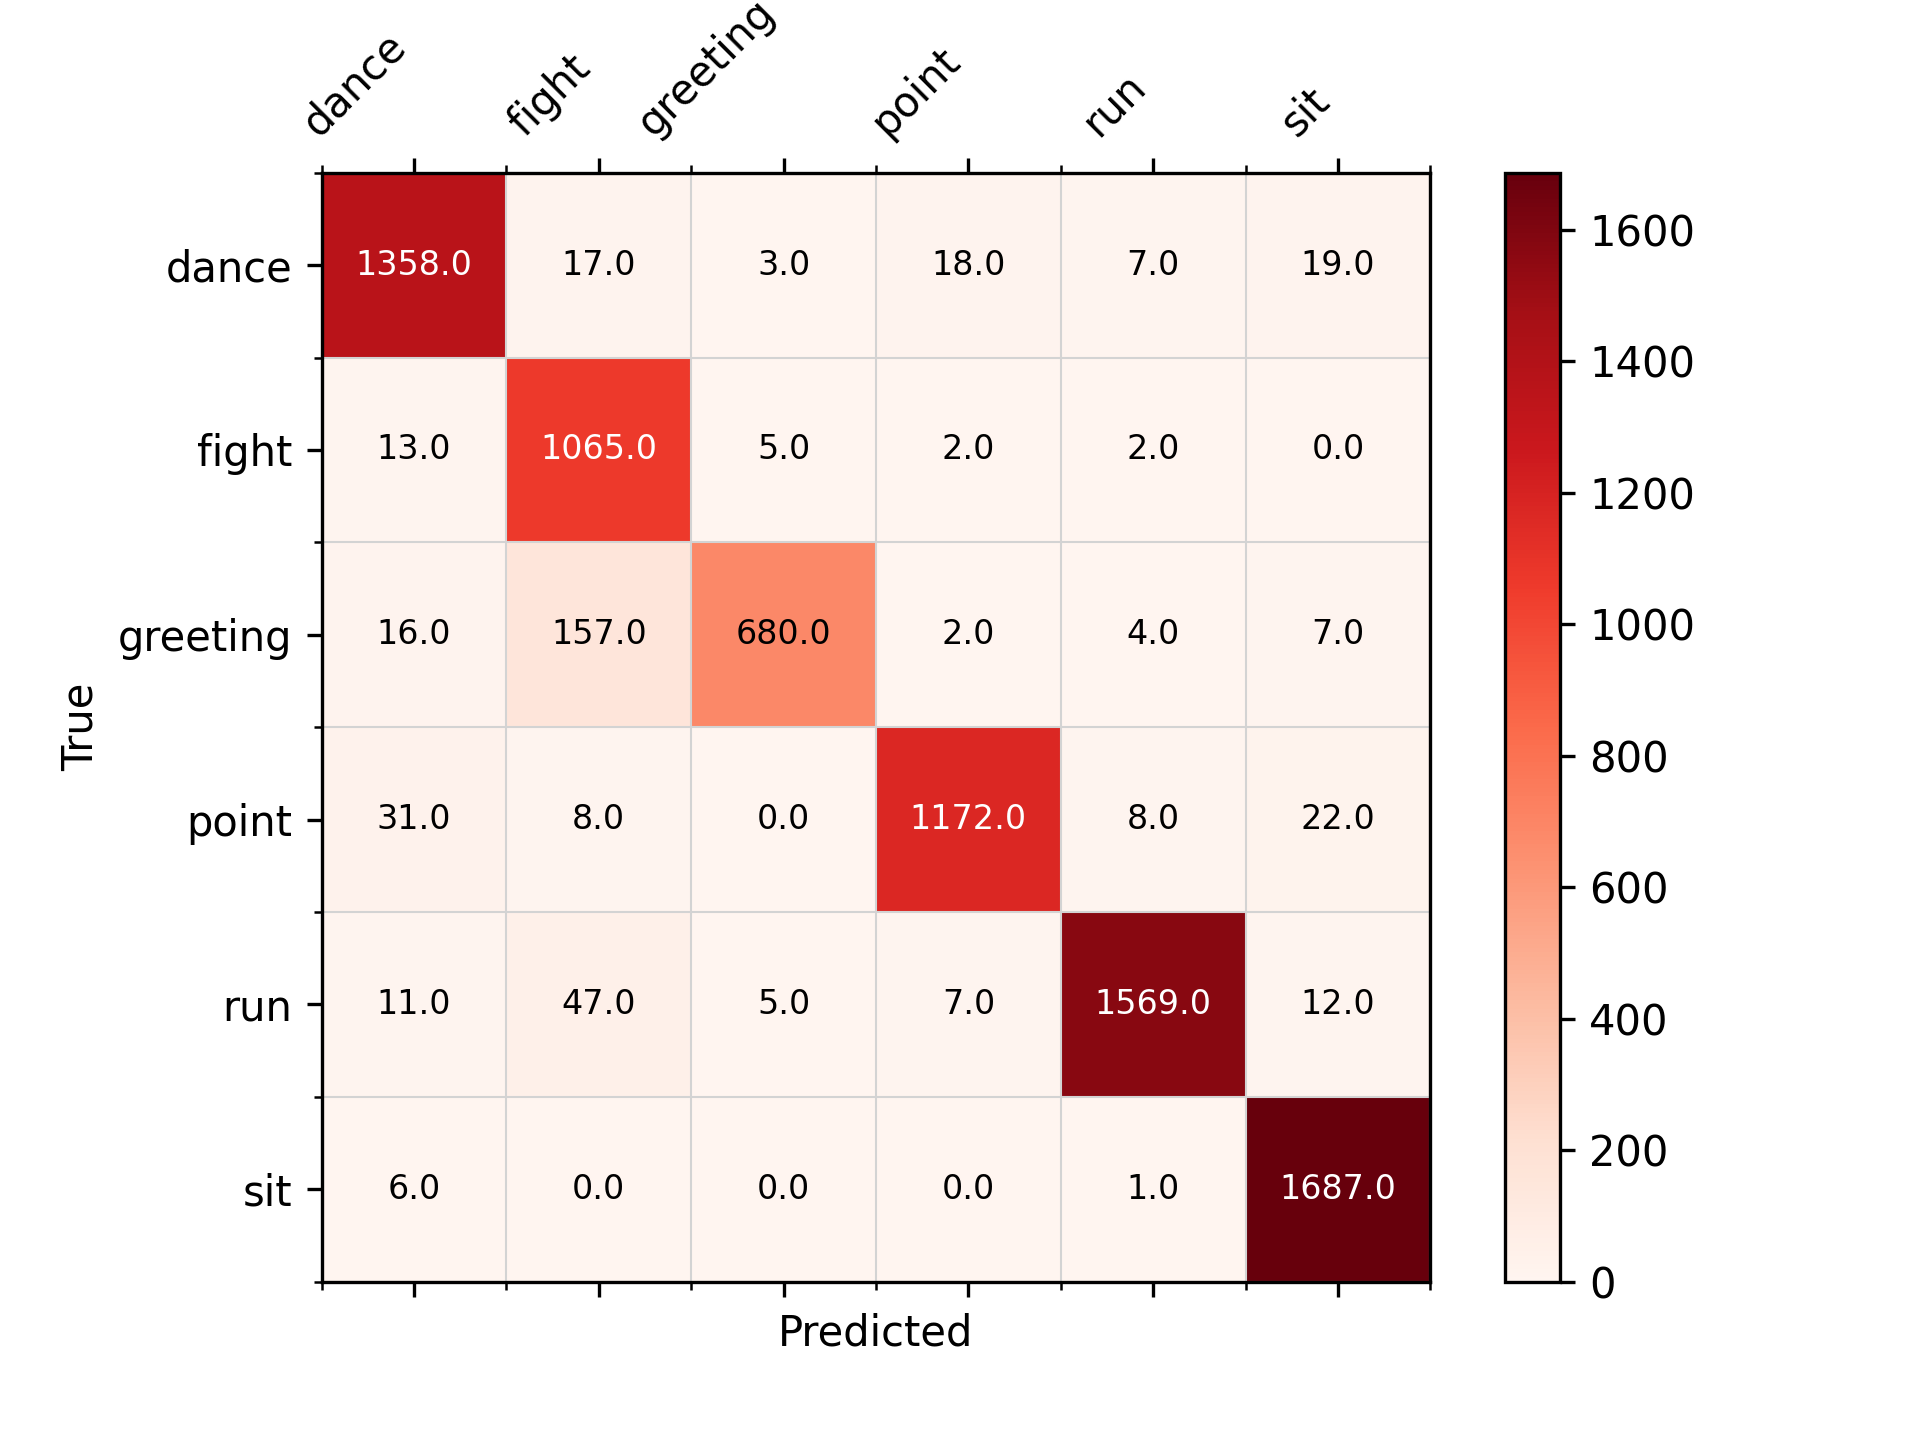
\includegraphics[width=0.6\textwidth]{Imagenes/Bitmap/CM_best_rf_0.8.png}
    \caption{Matriz de confusión del modelo RandomForest}
    \label{fig:rf-0.8-matriz-ejemplo}
\end{figure}

Este modelo finalmente es exportable a TensorFlow, siendo esto muy útil para su desplegado y compatibilización con otras herramientas. Dentro del repo, en la carpeta de ``notebooks'' se puede ver un resumen de las características más decisivas del modelo y su importancia en la diferenciación de dos gestos cuales sean.

\subsection{TensorFlow Serving}

Que todos los modelos sean exportables a TensorFlow permite el uso de TensorFlow Serving (\cite{olston2017tensorflowservingflexiblehighperformanceml}) para desplegar modelos. Serving nos proporciona una interfaz sencilla mediante \gls{API REST} para re entrenar los modelos y poder hacer inferencia sobre ellos desde cualquier máquina conectada a la red.

Este método de desplegado es especialmente útil a la hora de integrar los modelos con otras tecnologías sin necesidad de hace traducciones a otros lenguajes o formatos. El servidor se despliega usando docker y cogiendo el modelo de la última \textit{release} del repositorio. Para hacer una inferencia solo hay que hacer una petición \textit{POST} con el formato visto en la figura \ref{fig:ejemplo-petición} y el servidor devuelve la respuesta vista en la figura \ref{fig:ejemplo-respuesta}.

\begin{figure}[H]
    \centering
    \begin{lstlisting}[style=custombash]
curl <model_server>/v1/models/<model_name>:predict \
-X POST \
-d '{"instances": [{
    "feature_0":0.24,
    "feature_1":0.12,
    ... 
    "feature_599":0.56
}]}'
    \end{lstlisting}
    \caption{Ejemplo de petición a TensorFlow Serving}
    \label{fig:ejemplo-petición}
\end{figure}

\begin{figure}[H]
    \centering
    \begin{lstlisting}[style=custombash]
{
    "predictions": [{
        "scores": [0.981395662, 0.0186043456, 0.1920000, 0.0112349, 0.0001234, 0.0001234],
         "classes": ["dance", "fight", "greeting", "point", "run", "sit"]
    }]
}
    \end{lstlisting}
    \caption{Ejemplo de respuesta de TensorFlow Serving}
    \label{fig:ejemplo-respuesta}
\end{figure}

En el repositorio se pueden encontrar dos scripts, uno para windows y otro para linux, que permiten desplegar el servidor de manera automática siempre que docker ya esté instalado en el sistema.

\subsection{Hardware, complejidad de datos y otras limitaciones}

Este estudio ha estado muy limitado por el hardware disponible para el mismo. El equipo usado para el modelo tenía gráficas de consumidor de hace más de 5 años, haciendo que los modelos con redes neuronales tardaran bastante en entrenarse. Esto no fue un problema en el caso del \gls{randomforest}, ya que se entrena en \gls{cpu}.

Estas limitaciones de hardware también han afectado a la visión de los modelos a desarrollar, ya que en un principio se pensó en hacer modelos lo más simples posibles para poder utilizarlos incluso en equipos más limitados (gafas de \gls{vr} o equipos más antiguos).

Así mismo, la falta de espacios y de tiempo han resultado en que, junto a la falta de datasets ya formados, el número de datos fuera limitado para lo que requeriría el entrenamiento de redes neuronales.